\documentclass{article}
\usepackage[margin=25mm]{geometry} % 25 mm margins all around
\usepackage{hyperref} % for hyperlinks
\usepackage{enumitem} % for numbered lists
\usepackage{changepage} % for narrow margins on title
\usepackage{natbib} % for bibliography stuff
\usepackage{indentfirst} % allows subsections to be indented
\usepackage{mathtools} % for math stuff
\usepackage{graphicx} % for pdf figures

\bibliographystyle{vancouver} % sets bibliography format
\setcitestyle{numbers,open={[},close={]}} % sets in-text citation format. change later for isme.
\setcounter{secnumdepth}{0} % should get rid of section numbers

% regular expression for removing internal links:
% FIND: \\hyperref[.*?]
% REPLACE: \\label{.*?}

\begin{document}


{\parindent0pt % disables indentation on first page
\begin{adjustwidth}{1cm}{1cm} \begin{center}
\section{A phylogenetic model for the arrival of species into microbial communities and the human microbiome}
\end{center}  \end{adjustwidth}

\par
\textbf{Running Title}\\*
Phylogenetic community assembly of microbes
\\\par
\textbf{Authors}\\*
John L. Darcy\textsuperscript{1},
Alex D. Washburne\textsuperscript{2},
Michael S. Robeson\textsuperscript{3},
Tiffany Prest\textsuperscript{4},
Steven K. Schmidt\textsuperscript{4},
Catherine A. Lozupone\textsuperscript{1}
\\\par
\textbf{Affiliations}
\begin{enumerate}[topsep=0pt,itemsep=-1ex,partopsep=1ex,parsep=1ex, leftmargin=*,align=left]
	\item[\textsuperscript{1}] Department of Biomedical Informatics and Personalized Medicine, University of Colorado School of Medicine, Aurora, Colorado, USA.
	\item[\textsuperscript{2}] Department of Microbiology and Immunology, Montana State University. Bozeman, Montana, 59717, USA.
	\item[\textsuperscript{3}] Department of Biomedical Informatics, University of Arkansas for Medical Sciences. Little Rock, Arkansas, 72205, USA.
	\item[\textsuperscript{4}] Department of Ecology and Evolutionary Biology, University of Colorado. Boulder, Colorado, 80309, USA.
\end{enumerate}
\ \par
\textbf{Corresponding Author}\\*
J.L. Darcy; \href{mailto:darcyj@colorado.edu}{darcyj@colorado.edu}.
\\\par
\textbf{Conflict of Interest Statement}\\*
The authors declare that no conflict of interest exists.\\
\\
\textbf{Support}\\*
Funding was provided by an NSF grant for studying microbial community assembly following disturbance (DEB-1258160) and by a NIH NLM Computational Biology training grant (numbers go here, ask Elizabeth or Larry?). The funding bodies had no role in study design, analysis, interpretation, or in the preparation of this manuscript.\\

} % closing indentation remover

\newpage

% COVER PAGE ENDS HERE, BEGIN PAPER

% ABSTRACT
{\parindent0pt \section{Abstract}}
Understanding when and why species join microbial communities is a formidable problem. Much theory in microbial temporal dynamics is focused on how phylogenetic relationships between microbes impact the order in which those microbes join communities; for example species that are closely related may exclude each other due to high niche overlap. However, several recent human microbiome studies have instead found that close phylogenetic relatives often join microbial communities in short succession, suggesting factors such as shared adaptation to similar environments plays a stronger role than competition. To address this, we developed a mathematical model that describes the probabilities of different species joining a community over time, within a phylogenetic framework. We use our model to test three hypothetical assembly modes: underdispersion (species are more likely to join a community if a close relative has been previously observed), overdispersion (likelihood of joining is higher if a close relative has not been previously observed), and the neutral model (likelihood of joining is not related to phylogenetic relationships among species). We applied our model to longitudinal high-throughput sequencing data from the human microbiome, and found that the human microbiome generally follows an assembly pattern characterized by phylogenetic underdispersion. Exceptions were oral communities, which were not significantly different from the neutral model in either of two individuals analyzed, and the fecal communities of two infants that had undergone heavy antibiotic treatment. None of the data sets we analyzed showed statistically significant phylogenetic overdispersion.
\\\par

% INTRODUCTION
{\parindent0pt \section{Introduction}} \label{sec:introduction}
Every non-sterile surface in the world is in some stage of community assembly, from a forest of tropical trees to the microbes in a mammalian gut. The communities of organisms inhabiting these environments are dynamic through time, and studying patterns of assembly may shine light on general rules that govern their change. Understanding these community assembly rules may aid habitat restoration \cite{Palmer1997,Temperton2004}, the management of ecosystems that have undergone disturbances \cite{Richards1999,Bengtsson2000}, and ecological theory of phylogenetic signatures in community assembly \cite{ODwyer2012,Goberna2014}.Patterns and rules of community assembly are particularly important in human systems, including the primary succession of microbes on a human host following birth \cite{Koenig2011}, secondary successions following disease \cite{Frank2007,David2014}, disturbances caused by host lifestyle or antibiotic use \cite{Peterfreund2012,Kennedy2016,Guittar2019}, and the natural turnover of microbial communities over time \cite{Caporaso2011}. Insights into these difficult-to-observe community assembly processes can be gained via the comparison of microbial communities using high-throughput DNA sequencing \cite{Caporaso2011,Nemergut2013,Nemergut2016}, especially in longitudinal (time-series) studies \cite{Caporaso2011,Koenig2011,Kennedy2016}.
\par
A central question in microbial community assembly is when and why microbes join communities, which can be studied in part by evaluating the order in which particular microbes join communities given data such as which microbes are already present or what changes occur in an environment over time \cite{Nemergut2013,Sprockett2018}. Although the local environment clearly selects for microbial species, it has also been shown that microbial community structure is often historically contingent on previous states of that community \cite{Nemergut2013,Fukami2015,Sprockett2018,Verster2018,Litvak2019}. This reflects not only that microbial communities are temporally autocorrelated (gradual change over time), but also that the recruitment of a given species is a function of which species in the community are already present or have modified the local environment. Such historically contingent patterns have mainly been observed and tested within a phylogenetic context, because amplicon data naturally lend themselves to the creation of phylogenies, and because phylogenies have been shown to be predictive of genomic (and perhaps niche) overlap in human associated microbiota \cite{Zaneveld2010,Langille2013}.
\par
Within this phylogenetic framework, a predominant hypothesis has been that closely related microbes inhibit each other’s successful recruitment \cite{Nemergut2013,Fukami2015,Verster2018}. The proposed mechanism for this hypothesis is that closely related microbes likely have similar niches (phylogenetic niche conservatism \cite{Losos2008}), and the microbe that arrives first into a community will occupy its niche to the exclusion of ecologically similar strains. This is also the basis of Darwin’s naturalization hypothesis \cite{Darwin1859}, which proposed that species are less likely to join a community if a close relative is present \cite{Ma2016}. Indeed, this assembly mode has been found to be the case in artificial nectar microcosms, where phylogenetically similar yeast species had similar nutrient requirements, and inhibited each others’ colonization \cite{Peay2012}. In this paper, we refer to the assembly mode where distant relatives are more likely to join a community than close relatives as the \textbf{overdispersion hypothesis}, since it predicts the preferential addition of novel phylogenetic diversity to a community (\emph{i.e.} phylogenetic overdispersion).
\par
However, overdispersion is far from universal, and multiple studies have shown that extremely close relatives can coexist within the human microbiome \cite{Li2016}, and may even be preferentially recruited \cite{Brown2018}. Indeed, Darwin’s pre-adaptation hypothesis predicts that species with a close relative present in a community will be preferentially recruited, because they are likely to already be adapted to the new environment \cite{Darwin1859}. This hypothesis predicts that close relatives are more likely to join a community than distant relatives, so the amount of new phylogenetic diversity added to a community is minimized (phylogenetic underdispersion). For this reason, we refer to this hypothesis as the \textbf{underdispersion hypothesis}. Both this and the overdispersion hypotheses are alternatives to the null hypothesis that species arrival into communities is independent of phylogenetic relatedness among species. Since the null hypothesis is species-neutral (and phylogenetically neutral), we refer to it as the \textbf{neutral hypothesis}.
\par
Here, we use the phylogenetic relationships among species within a time-series to understand the community’s change over time in a new way. Instead of analyzing broad patterns of community change via beta-diversity statistics (\emph{e.g.} UniFrac \cite{Lozupone2005}) or analyzing patterns of select clades within the community (\emph{e.g.} PhyloFactor \cite{Washburne2017}, Edge PCA \cite{Matsen2013}), we model the probability of each new species’ first arrival into the community as a monotonic function of its phylogenetic distance to members of the community that have already arrived.
\par
The model we present here can be used to estimate the degree to which newly arriving species are phylogenetically over- or underdispersed during a time-series microbiome dataset. Said another way, we estimate the extent to which these arrival events are “nepotistic”, meaning species are more likely to arrive when a close relative is already present (phylogenetic underdispersion). We fit our model (described in our methods section, below) to several time-series human microbiome data sets \cite{Caporaso2011,Koenig2011,Yassour2016}, to compare patterns of microbial community assembly between subjects, sample sites, or time periods. We found that in general, the human microbiome follows the underdispersion hypothesis – microbes with low phylogenetic distance to the existing community had a higher probability of recruitment than microbes with a high phylogenetic distance to the existing community. There were exceptions where this pattern was not significantly different than the neutral model, but none of the longitudinal data sets we analyzed showed statistically significant overdispersion. Furthermore, the predominance of non-neutral assembly in the microbial communities analyzed here suggests that phylogeny carries relevant and potentially predictive information for microbial community assembly, with implications for microbiome perturbation and rehabilitation. 
\\\par



% METHODS
\section{Materials and Methods}

\subsection{Overview} \label{sec:overview}
Here, we describe a statistical model of phylogenetic microbial community assembly, and how we apply that model to time-series microbiome data. Our goal is to estimate the degree to which species arriving into a community for the first time are phylogenetically over- or underdispersed, competitively testing the overdispersion or underdispersion hypotheses against the neutral hypothesis. Said another way, we want to estimate the extent to which recruitment of species into the community is related to arriving species’ phylogenetic similarity to (or distance from) species that already arrived. Our \hyperref[sec:statisticalModel]{\textbf{Statistical Model}} describes the probabilities of those species arriving into a community over time. We use our model with empirical data via \hyperref[sec:simulations]{\textbf{Simulations}}, where we re-sample the empirically observed species using our model with known parameter values, to produce surrogate data sets. Specifically, we fix and record the model’s dispersion parameter (D), which determines the extent to which species with a close relative are preferentially added to the surrogate community (or, conversely, if species without a close relative are preferred). Our \hyperref[sec:parameterEstimation]{\textbf{Parameter Estimation}} compares the empirical pattern of species arrival to that of the surrogate data sets (which have known D values), in order to determine which value of D best describes the empirical data. \hyperref[sec:hypothesisTesting]{\textbf{Hypothesis Testing}} is done by comparing empirical data to repeated simulations under the neutral model, which is D = 0. We describe the bioinformatic and technical details of this process in our \hyperref[sec:analysis]{\textbf{Analysis}} section, and make our code available to others in the \hyperref[sec:codeAndData]{\textbf{Code and Data}} section. 

\subsection{Statistical Model} \label{sec:statisticalModel}
At any point in time, a community is composed of many species, and other species are not present but are available to be added. Species not yet added (“species pool”) represent organisms present within the metacommunity but not the local community. Our model parameterizes the probability of species arriving in a local community for the first time, based on their phylogenetic distances from species that have already arrived. In a species-neutral model of community assembly, each species \(i\) in the species pool has the same probability of arrival at time \(t\), irrespective of how different it is from species that are already present at time \(t\). Thus, the neutral model for first-time arrivals is a random draw without replacement of species from the species pool. We extend the species-neutral model by modeling the probability \(p_{i,t}\) of species \(i\) being observed for the first time at time \(t\) as,
\begin{equation}
	\label{sec:equation1}
	p_{i,t} = \frac {d_{i,t}^D} { \sum\limits_{\hat{i}} d_{\hat{i},t}^D } 
\end{equation}
where \(d_{i,t}\) is the phylogenetic distance from species \(i\) to its closest relative that has already been observed prior to time point \(t\), and \(D\) is a dispersion parameter.
\par
When \(D = 0\), our model functions as a neutral model; all species have the same probability of arriving in the community for the first time, since pi,t is the same for every species. When \(D < 0\), \(p_{i,t}\) decreases with \(d_{i,t}\) meaning that species from the species pool have higher probabilities of arriving when they are more closely related to species that have already been observed in the local community (underdispersion; phylogenetically constrained). When \(D>0\), the opposite is true (overdispersion; phylogenetically divergent). Our hypothesis testing and parameter estimation focus on the dispersion parameter, \(D\).

\subsection{Simulations} \label{sec:simulations}
Our analysis of a data set relies on re-constructing that data set via simulation of our statistical model using known values of \(\hat{D}\), allowing for hypothesis testing and parameter estimation (we refer to the empirical dispersion parameter as \(D\), and use \(\hat{D}\) to refer to surrogate values used in simulations). Using the empirical data as a starting point, we simulate many surrogate data sets with \(\hat{D}\) values ranging from \(\hat{D}<0\) (underdispersed) to \(\hat{D}=0\) (neutral) to \(D>0\) (overdispersed). This is done so that the empirical data can later be compared to the surrogate data sets, to estimate the empirical value of \(D\).
\par
We start each surrogate data set with the same species present in the first sample of its corresponding empirical data set. Then, surrogate data sets are constructed forward in time by randomly drawing \(r_t\) new arrivals from the species pool (all species observed in the empirical data set that have not yet been sampled by this process), where the probabilities of species arriving at any given time are given by  \hyperref[sec:equation1]{Equation 1}, and \(r_t\) is the number of new arrivals in the empirical data set from times \(t-1\) to \(t\). The number of arrivals from the empirical data set is used so that species richness is kept constant between the empirical data set and all surrogate data sets. The species pool is updated to exclude those species drawn at previous time points, and the newly sampled species are recorded. Surrogate data sets are produced for many different \(\hat{D}\) values, ranging from underdispersed to overdispersed models. In the analyses we present here, we performed 500 simulations (as described above) for each data set analyzed.

\subsection{Parameter Estimation} \label{sec:parameterEstimation}
Our main goal is to estimate the empirical dispersion parameter \(D\) (\hyperref[sec:equation1]{Equation 1}), which quantifies the degree to which first-time arrivals are phylogenetically underdispersed (\(D<0\)), neutral (\(D=0\)), or overdispersed (\(D>0\)). As previously stated, these assembly modes correspond to our hypotheses (see \hyperref[sec:introduction]{Introduction} section). To this end, we use Faith's phylodiversity \cite{Faith1992} to compare each of the 500 surrogate data sets (described above) to the empirical data set. Phylodiversity is the sum of branch-lengths on a phylogenetic tree for a set of species, so phylodiversity of a set of highly related species is low (phylogenetically constrained) because there are no long branch lengths in the tree, but phylodiversity is higher (phylogenetically divergent) for a set of more distantly related species \cite{Faith1992}. If \(D\neq0\), then species are preferentially added if they have relatively low (\(D<0\)) or relatively high (\(D>0\)) phylogenetic distance to the resident community (\(d_{i,t}\), \hyperref[sec:equation1]{Equation 1}), yielding accumulations of total phylodiversity that are relatively slow (\(D<0\)) or relatively fast (\(D>0\)) compared to the neutral model (\hyperref[sec:figure1]{Figure 1A}). In other words, at any time point \(t\), the phylogenetic diversity of species that have already been observed is \(PD_t\), and the extent to which \(PD_t\) accelerates or decelerates over a sampling effort depends on \(D\). Because of this, we can estimate \(D\) by comparing the empirical phylodiversity curve to our surrogate phylodiversity curves, which have known \(\hat{D}\) values.
 \par
For the comparison of an empirical phylodiversity accumulation curve to curves for corresponding surrogate data sets, we evaluate the amount of phylodiversity \(PD_m\) accumulated at time index \(m\), midpoint between the first and final samples. Time \(m\) is used because this leaves many species yet to be observed in the species pool, so that there can be variability in surrogate data sets. Multiple time indices are not used to compare surrogate and empirical data sets because each value \(PD_{\hat{t}}\) is a function of all values \(PD_{t<\hat{t}}\). \(PD_m\) values are calculated for all surrogate data sets, and a \(PD_m\) value is calculated for the empirical data set. The differences between the empirical \(PD_m\) and each \(PD_m\) simulated with \(D=\hat{D}\) are given by the vector \(\Delta PD_{\hat{D}}\), which is the error between surrogate and empirical data. We then estimate the empirical value of \(D\) by minimizing \(\Delta PD_{\hat{D}}\) (\hyperref[sec:figure1]{Figure 1B}). This minimization is performed using a logistic error model,
\begin{equation}
	\label{sec:equation2}
	\Delta PD_{\hat{D}} = \frac {a-b} { 1 + e^{-r(\hat{D} -i)} } + b 
\end{equation}
where \(a\) and \(b\) are the upper and lower horizontal asymptotes, and \(r\) and \(i\) are rate and inflection parameters for the logistic model. \(\Delta PD_{\hat{D}}\) is modeled with a logistic function because there is a maximum and minimum observable \(\Delta PD_{\hat{D}}\) value as a function of the phylogeny; this is because there are strict minimum and maximum limits to the amount of phylodiversity obtainable by observing \(n\) species where \(n\) is the total species richness accumulated up to time \(m\). The two horizontal asymptotes of the logistic model are easily fit to these extremes (\hyperref[sec:figure1]{Figure 1B}). Once fit, the error model is solved for \(\Delta PD=0\), giving an estimate for the empirical \(D\). Confidence intervals for this estimate are obtained via bootstrapping our error model.

\subsection{Hypothesis Testing} \label{sec:hypothesisTesting}
For this test, our null hypothesis is the neutral model, where \(D = 0\), since this model represents the absence of the effect we are testing (over- or underdispersion, a 2-tailed test). We test this null hypothesis competitively by simulating 1000 surrogate data sets at \(D = 0\) (\hyperref[sec:figure2]{Figure 2A}) to generate a null \(PD_m\) distribution. The empirical \(PD_m\) is compared to this distribution (\hyperref[sec:figure2]{Figure 2B}), and if the empirical \(PD_m\) is below the 2.5\% quantile or above the 97.5\% quantile, we reject the null (\emph{i.e.} neutral) hypothesis. Evidence of either overdispersion (\(D > 0\)) or underdispersion (\(D < 0\)) allows us to reject.

\subsection{Analysis} \label{sec:analysis}
Infant gut 16S rDNA sequencing data from Koenig \emph{et al.} \cite{Koenig2011} were downloaded from the NCBI Short Read Archive (SRA) website (\url{http://www.ncbi.nlm.nih.gov/sra}) along with their metadata. These data are a time-series of fecal bacterial communities from an infant subject, over the first 500 days of life. QIIME \cite{Caporaso2010} was used to trim primer regions from these data. Clustering was performed using the unoise3 pipeline \cite{Edgar2016}; sequences were de-replicated at 100\% identity using vsearch \cite{Rognes2016}, zOTU centroid sequences were picked and chimeric sequences were removed using unoise3 \cite{Edgar2016}, then all sequences were mapped onto zOTU seeds to create a zOTU table using vsearch. zOTU stands for “zero-radius operational taxonomic unit” \cite{Edgar2016}. Unlike traditional de novo clustered OTUs, zOTUs are exact sequence variants (ESVs) which are consistent and easily comparable across data. The SINA aligner \cite{Pruesse2012} was used to align zOTU centroid sequences to the SILVA SSU Ref 128 database (available from \url{https://www.arb-silva.de/download/arb-files/}). We then used IQ-TREE \cite{Nguyen2015} to build a phylogenetic tree from the aligned sequences.
\par
The resulting zOTU table was rarefied to 1000 sequences per sample, and samples with fewer sequences were excluded. The last five time points were excluded as well because they were sampled at a much lower temporal resolution. This left 52 time points spread over the first 469 days of the infant subject's life. The zOTU table was then split into two zOTU tables, one for time points before the infant started consuming baby formula, and one for those after. The “pre-formula” zOTU table contained ages 4 days through 146, and the “post-formula” zOTU table contained ages 161 days through 469 days. Each zOTU table was used to run our model as described above using 500 D values (\hyperref[sec:equation1]{Equation 1}), ranging from underdispersed (\(D = -5\)) to overdispersed (\(D = 5\)), using zOTUs in lieu of species. zOTUs with zero phylogenetic distance between them were combined, because these zOTUs were uninformative for our statistical model (\hyperref[sec:equation1]{Equation 1}; zero raised to a negative exponent is undefined). The 500 resulting surrogate data sets were compared to the empirical data set as described above, using difference between phylodiversity values at the middle time point. The logistic error model (\hyperref[sec:equation2]{Equation 2}) was fit and bootstrapped, yielding an estimate for \(D\) and 95\% confidence intervals for that estimate.
\par
“Moving pictures” sequence data from Caporaso \emph{et al.} \cite{Caporaso2011} were downloaded from the MG-RAST database (\url{http://metagenomics.anl.gov/}). These are longitudinal data from one adult male subject and one adult female subject, over a period of several hundred days, across multiple sample sites (feces, both palms, tongue). Time points were excluded which did not have sequence data for each of the 8 environments (L hand, R hand, mouth, and feces of the male and female subjects), and rarefied to 5000 sequences per sample. This left 107 time-points, ranging from day 1 to day 185. Analysis for each data set (e.g. female right palm) was carried out as described above, except raw sequences were trimmed to a length of 91 bp after the end of the forward PCR primer site in order to ensure that all raw sequences spanned the same region of the 16S rRNA gene. 91 bp was chosen as a length cutoff in order to keep 95\% of the sequence data (5\% of sequences were discarded because they were shorter).
\par
Analysis of the “moving pictures” data was also done using two approaches that were intended to showcase potential functionality of our model, albeit without directly testing any hypotheses. We analyzed palm communities in a “meta” context, where surrogate data sets were generated assuming the species pool for a given palm was composed of all four palms in the data set. In this case, the difference between the “self” \(D\) estimate (generated above) and the “meta” \(D\) estimate (estimated with a metapopulation of zOTUs) is related to the exclusivity of arrivals into the community. In other words, if we were to estimate similar \(D\) values for both the “meta” and “self” analyses, the inclusion of extra species in the species pool would be of little importance to the model, and we would learn that it would make little difference to community assembly patterns if the species pool really was composed of the “meta” set. We also analyzed a section of samples from the male right palm data that were collected every day over a period of 19 days, using a sliding window approach. We ran our model as described above on each window of 5 continuous days (15 windows), in order to see how \(D\) varied over time. We only conducted this analysis for the section of samples that were sampled every day, so that comparisons between windows would not be confounded by window size.
\par
Finnish infant sequence data from Yassour \emph{et al.} \cite{Yassour2016} and associated metadata were downloaded from the DIABIMMUNE Microbiome Project website (\url{https://pubs.broadinstitute.org/diabimmune}). These are longitudinal gut microbiome data from Finnish infants, collected over the first 36 months of life \cite{Yassour2016}. Roughly half of these infants were repeatedly treated with oral antibiotics, almost universally for ear infections. Metadata for this data set were compiled in a different re-analysis of these data \cite{Guittar2019} and were downloaded from the authors’ GitHub page (\url{https://github.com/ShadeLab/microbiome_trait_succession}). Subject data sets belonging to the groups “Antibiotic” (\(n\)=18) or “Control” (\(n\)=15) were each analyzed using our model, similar to above. These subjects had between 19 and 36 samples collected over 36 months, with a mean of 28 samples. Sequence data were rarefied to 5000 sequences, and our model was run per above. We compared the estimated \(D\) values between antibiotic and control groups using a Mann-Whitney test. Because this data set had so many subjects, we used this analysis as an opportunity to analyze whether the number of zOTUs, total phylodiversity, or number of time-points had an effect on estimated \(D\) values. This was done via correlation analysis of \(D\) estimates with the aforementioned potential covariates.

\subsection{Code and Data} \label{sec:codeAndData}
R code and data to replicate our analysis, or to perform a similar analysis on other data, are available at \url{https://figshare.com/s/922b268891f1945c1944} (temporary private link, please do not share until publication). R functions to use our model are also available on GitHub, along with a tutorial vignette: (link will be added upon acceptance).


% RESULTS
\section{Results} \label{sec:results}
By varying \(\hat{D}\), we successfully changed the rate at which phylodiversity is added to surrogate (\emph{i.e.} resampled) microbial communities over time (\hyperref[sec:figure1]{Figure 1A}). Compared to the neutral model where \(\hat{D} = 0\), higher \(\hat{D}\) values result in phylodiversity accumulating quickly, since in the overdispersed model, species that contribute more phylodiversity are preferentially sampled. Conversely, lower \(\hat{D}\) values result in phylodiversity accumulating slowly, since in the underdispersed model, species that contribute less phylodiversity (since they are very similar to species that are already present) are preferentially sampled. These results show that the \(D\) parameter in our model successfully corresponds to over- and underdispersion relative to the neutral model. Our error model also fit nicely to the differences between empirical and surrogate data sets (\(\Delta PD_{\hat{D}}\), \hyperref[sec:figure1]{Figure 1B}). Each error model fit was manually inspected to be sure that \(D\) estimates were not spurious, and all data analyzed produced nice looking fits, including data sets where \(D\) was not significantly different from 0. 

\subsection{Results from “moving pictures” data}
All time-series from adult feces and palm microbiomes \cite{Caporaso2011} showed significant phylogenetic underdispersion of first-time arrivals (\hyperref[sec:figure2]{Figure 2}). This means that when a zOTU was observed for the first time in one of these communities, it was more likely to be phylogenetically similar to a zOTU that had previously arrived in that community. For both the male and female subject, \(D\) estimates were lower (more underdispersed) in the feces than in the palms, left and right palm \(D\) estimates were similar to each other, and tongue \(D\) estimates were higher. All sites except the tongue showed statistically significant underdispersion in both subjects, while tongue data were not significantly different than the neutral model. In the comparison between “meta” and “self” models, “meta” models needed to be much more underdispersed than “self” in order to approximate empirical phylogenetic diversity accumulation (\hyperref[sec:figureS2]{Supplemental Figure 2}). We also observed a general upward trend in \(D\) in our sliding window analysis of the male right palm data set (\hyperref[sec:figureS3]{Supplemental Figure 3}), although this trend was only observed over 19 days.

\subsection{Results from infant gut data}
Empirical phylodiversity accumulation in the infant gut microbiome \cite{Koenig2011} showed a sharp increase in phylodiversity after day 161 (\hyperref[sec:figure3]{Figure 3}), the same date that the subject began consuming baby formula. This suggests that baby formula changed the phylogenetic colonization patterns of the developing infant gut. We analyzed this data set as two separate time-series, one before formula use and one during, and both had negative \(D\) estimates, with the pre-formula \(D\) estimate being lower (\hyperref[sec:figure4]{Figure 4}). While the pre-formula data set was significantly underdispersed (\(P = 0.007\)), the formula data set was not significantly different from the neutral model, although this result is marginal (\(P = 0.107\)). Infant gut data from Finnish infants \cite{Yassour2016} were sampled at a much lower temporal resolution, and as such were not split between formula use. 31 out of 33 individuals analyzed exhibited significantly significant underdispersion, and the other two were not significantly different from the neutral model. Both nonsignificant individuals were from the group treated with heavy antibiotics, but even so, no significant difference in \(D\) values was detected between antibiotics and control groups (\hyperref[sec:figureS4]{Supplemental Figure 4}). Estimates of \(D\) did not significantly correlate with the number of zOTUs in a data set, the total phylodiversity of the data set, or the number of samples in a data set (\hyperref[sec:figureS5]{Supplemental Figure 5}). 


% DISCUSSION
\section{Discussion}
Any organism of interest in a human microbiome data set, from the pathogenic to the probiotic, will at some point arrive for the first time, 
and the order in which these organisms arrive 
in the community is determined by community assembly 
processed \cite{Nemergut2013}. Predicting which lineages of organisms can be recruited into a given environment has far-reaching implications for ecosystem remediation and management, especially in microbial communities where the medical and ecological importances of many microbes are still largely unknown \cite{Martiny2015,Vazquez-Baeza2018}. Identifying conditions under which assembly mechanisms change, or under which non-neutral assembly is particular strong, may facilitate microbial community rehabilitation by understanding when and how microbial communities can be colonized by close/distant relatives. If there are patterns or general rules for which taxa have higher probabilities of arriving, these rules can guide habitat restoration projects, help us better design probiotics for colonization, and better exploit disturbance as a tool for managing microbial systems related to human health and disease. We found that assembly during primary succession of the infant gut (\hyperref[sec:figure4]{Figure 4}, \hyperref[sec:figureS4]{Supplemental Figure 4}) and during turnover of the microbial communities on the adult palms and gut (\hyperref[sec:figure2]{Figure 2}) follows a predictable pattern: species are more likely to arrive if a close relative has already arrived.
\par
This generally “nepotistic” pattern in arrivals strongly supports our underdispersion hypothesis, which is similar to Darwin’s pre-adaptation hypothesis \cite{Darwin1859}. Under that hypothesis, species are better able to join a community where a close relative is present because they likely already have the “right stuff” to live there. This is because closely related species are likely to be ecologically similar due to phylogenetic niche conservatism \cite{Wiens2010}. Although the phylogenetic trees we use here are constructed with 16S rDNA sequences, such phylogenies have been shown to track genomic differences in bacteria \cite{Zaneveld2010,Langille2013}. Indeed, non-neutral patterns of phylogenetic community structure have been interpreted to mean that traits are under ecological selection \cite{Webb2000,Webb2002,CavenderBares2004,Gerhold2015}. If traits are not driving community assembly \cite{Hubbell2001} or if the traits driving community assembly are largely horizontally transferred between taxa independent of their relatedness (as estimated by a 16S rDNA phylogeny), we would expect no phylogenetic signature, and a \(D\) estimate that is not significantly different from 0 (the neutral model). Instead, we observed very a strong and significant phylogenetic signal in arrival order for almost all data sets we analyzed.
\par
However, even if microbial community assembly follows the pre-adaptation hypothesis, selection itself may not occur within the host environment. An alternative explanation for the underdispersion we observed is that selection is external to the host environment (\emph{i.e.} selection occurs within the neighboring species pool from which emigration occurs), causing change in the community entering the host to already be underdispersed. Similarly, phylogenetic dispersion of community structure has been unable to distinguish between selection and differences in migration rates \cite{Emerson2008}, so a pre-underdispersed community entering the host is a plausible mechanism for phylogenetic underdispersion of arrivals. But selection of microbial communities within the host has been shown by multiple studies \cite{Peterfreund2012,David2014,Kennedy2016}, so it is our opinion that selection within the host is a more likely scenario.
\par
As to why no data sets analyzed showed significant phylogenetic overdispersion (\(D > 0\)), we are not certain. At the beginning of development of this model, we expected microbial communities in the human microbiome to follow the overdispersion hypothesis, partly from our own intuition, and also because of work in experimental microcosms supporting Darwin’s naturalization hypothesis \cite{Peay2012}. However, the human microbiome environments analyzed here are environments that undergo constant physical disturbance, unlike aqueous microcosms. Palm communities are physically disturbed with every use of the hands, and by the sampling procedure itself. Gut (fecal) communities are also disturbed constantly by the movement of feces through the gut. It may be possible that continuous disturbance allows for underdispersion or Darwin’s pre-adaptation hypothesis via constant re-assembly of communities. In this case, niches may be filled by random “winners” after each disturbance, as in a competitive lottery scenario \cite{Verster2018}. These “winners” would still need to be adapted to their environment, so they would be more likely to be closely related to previous “winners”, as in our findings. Analysis using our model captures pattern, but does not interrogate the process by which underdispersion occurs, and future experiments will need to be designed with such considerations in mind.
\par
Nonetheless, a strength of our model is that it estimates values of \(D\) that can be compared among data sets (\hyperref[sec:figure2]{Figure 2}) or potentially across time (\hyperref[sec:figure4]{Figure 4}, \hyperref[sec:figureS3]{Supplemental Figure 3}) in order to learn how differences between data sets impact community assembly. We found that gut and palm communities were almost universally underdispersed (\hyperref[sec:figure2]{Figure 2}, \hyperref[sec:figure4]{Figure 4}, \hyperref[sec:figureS4]{Supplemental Figure 4}), and that the D value for a community appears to be a function of body site (\hyperref[sec:figure2]{Figure 2}). Although this result is only shown across two subjects, the parallel patterns between the male and female subject are striking, in that fecal communities are the most strongly underdispersed (lowest \(D\)), palm communities are similar to each other, and tongue communities had the highest \(D\) estimates.  Similarly, comparing \(D\) before and after an event can be used within an experimental framework to see how that event may affect community assembly. Our analysis of infant gut microbiome data \cite{Koenig2011} before and during the use of baby formula (\hyperref[sec:figure4]{Figure 4}) showed that while the pre-formula community was significantly underdispersed, community assembly during formula consumption was more neutral. While the post-formula trend was not significantly different from the neutral model, this finding was marginal (\(P = 0.107\)). 
\par
In addition to showing that our model can be a useful tool for future studies, our findings also hint that phylogenetic underdispersion may be a general trend for the human gut microbiome, and potentially for skin microbiomes as well. If true, our findings have implications for the management and restoration of human-associated microbial systems \cite{Shooner2015}, in particular for probiotic development and remediation of pathological microbial communities. Without any other information, our finding of consistent phylogenetic underdispersion in arrivals suggests that probiotics for sustained colonization of the human gut should be close relatives to the microbes already present. Indeed, recent research has shown that for fecal transplants, donor strains are able to integrate into the recipient's gut community when a conspecific strain is already present, but novel donor strains are unlikely to successfully integrate into the recipient \cite{Li2016}. Different body sites - as we saw with the skin – may have qualitatively similar patterns of underdispersion, yet quantitatively different magnitudes of this effect. Thus the efficacy of an engineered probiotic based on similarity to organisms already present in the community for which it was engineered may largely depend on the body site for which it's intended.
\par
Microbial communities provide a unique opportunity to study community assembly in primary and secondary succession. In addition to standard cross-sectional studies of communities of different ages or successional stages, the short timescales of microbial community dynamics allows longitudinal studies of community assembly over manageable time frames \cite{David2014,Kennedy2016}. Microbial communities allow large sample sizes, longitudinal studies, and experimental manipulations that enable us to identify general rules and statistical patterns of community assembly. The model we present here makes use of such data, and to facilitate further discovery both in the human microbiome and in other environments, we have made our R code available at FigShare: \url{https://figshare.com/s/922b268891f1945c1944} (temporary private link, please do not share until publication) and GitHub: (link will be added upon acceptance).

% ACKNOWLEDGEMENTS
\section{Acknowledgements}
The authors thank D.R. Nemergut for her help and support, and also thank J.P. O'Dwyer, P. Sommers, E.M. Gendron, A. Solon, E. Preusse, K. Hazleton, and S. Sauce for many helpful discussions. 


% FIGURES
\newpage

\section{Figures}
{\parindent0pt % no indentation until closed
\begin{figure}[ht]
	\centering
	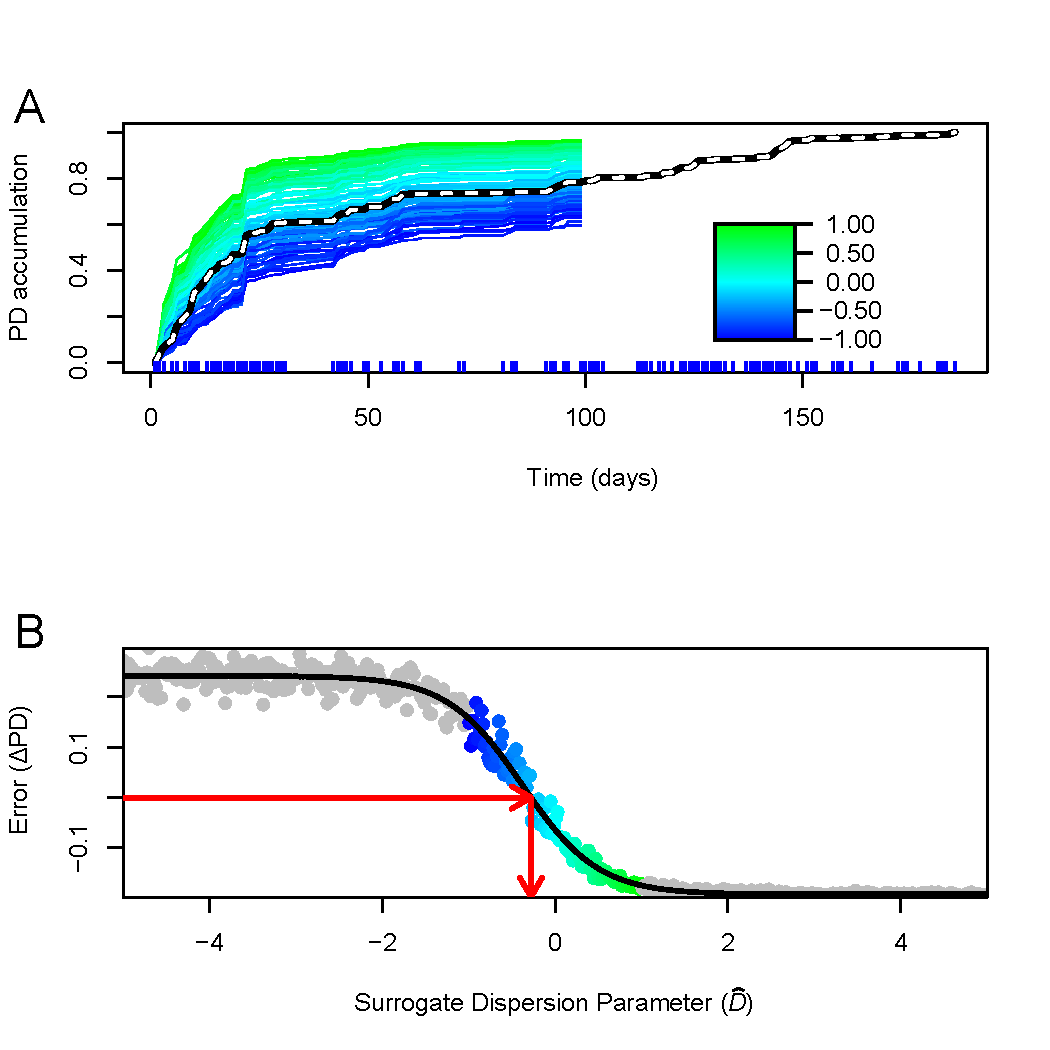
\includegraphics[scale=0.80]{figs/Fig_1.pdf}
\end{figure}
\textbf{Figure 1:}\label{sec:figure1} Phylodiversity accumulation and model fitting in the female feces data set \cite{Caporaso2011}. Plot A shows empirical (dashed) and surrogate phylodiversity accumulation curves. Each time point's phylodiversity value is the cumulative sum of all branch lengths observed up to that time point \cite{Faith1992}. Curves are rescaled from 0 to 1 in this figure. The colored lines are 500 surrogate (\emph{i.e.} resampled) phylodiversity curves with different \(\hat{D}\) values (\hyperref[sec:equation1]{Equation 1}), and are only calculated up to time point \(m\), which is used to compare empirical and surrogate values. These lines are color-coded by their \(\hat{D}\) value (see key at right). The empirical model (dashed) is below the neutral model (teal), signifying underdispersion in the order of first-time arrivals. The times of sampling points are shown as vertical blue lines below the X-axis. Plot B shows how empirical and surrogate data are compared to generate an estimate for \(D\). Differences between empirical and surrogate data at time \(m\) are shown on the Y-axis, and the \(\hat{D}\) values used to generate surrogate data sets are shown on the X-axis. Color-coded points correspond to surrogate data sets shown in plot A. Values shown in gray result from using extreme values of \(\hat{D}\), which help the logistic error model (black line) fit to the data, and are not shown in plot A. The red arrows show the process of solving the model for 0 error, yielding a \(D\) estimate. A figure showing significance testing for these data is available as \hyperref[sec:figureS1]{Supplemental Figure 1}.
\newpage

\begin{figure}[t]
	\centering
	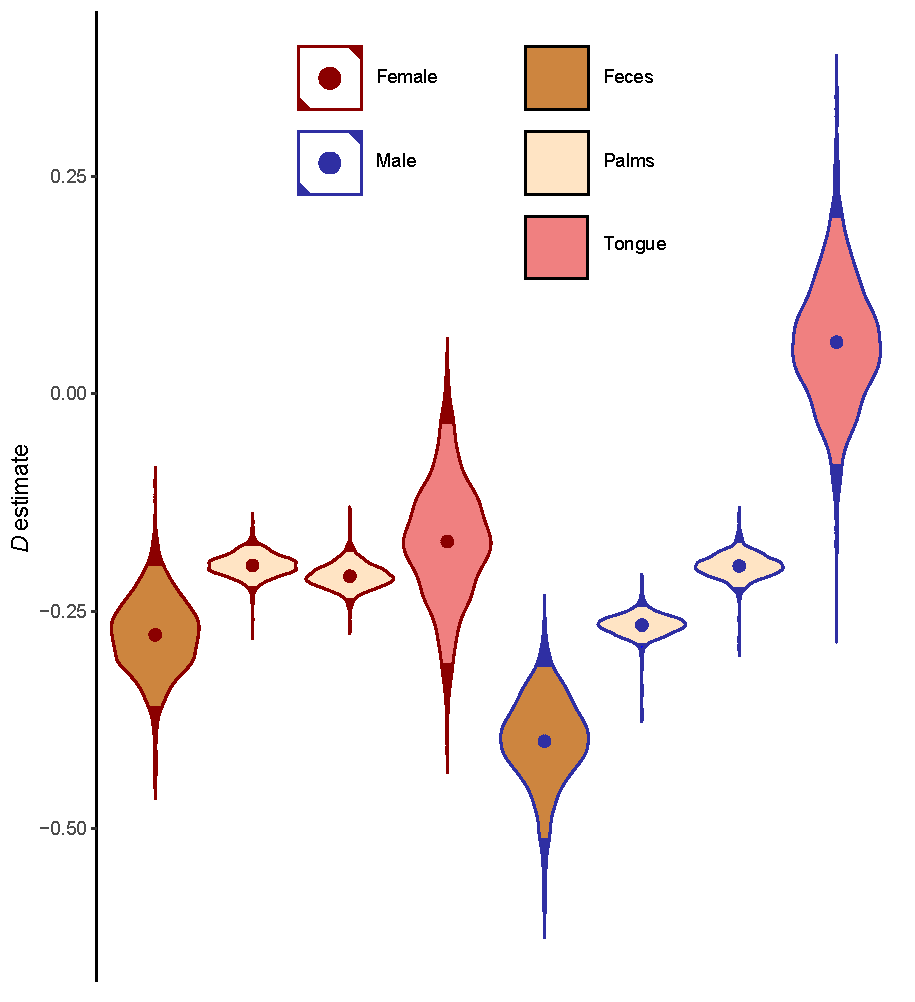
\includegraphics[scale=0.80]{figs/Fig_2.pdf}
\end{figure}
\textbf{Figure 2:}\label{sec:figure2} Dispersion parameter (\(D\)) estimates for “moving pictures” \cite{Caporaso2011} data sets. The subject’s sex is shown as the outline color of each violin, and the body site is shown as fill color. The four body sites for the female subject are shown at left, and the four body sites for the male subject are shown at right. Each viollin shows the distribution of \(D\) estimates given by logistic error model bootstraps, and the dots within violins are means. Colored portions of violins represent 95\% of bootstraps. The two subjects analyzed show parallel \(D\) estimates, with feces being the lowest, followed by palms which are all similar, followed by tongue communities. For both subjects, tongue patterns were not significantly different than the neutral model.
\newpage

\begin{figure}[t]
	\centering
	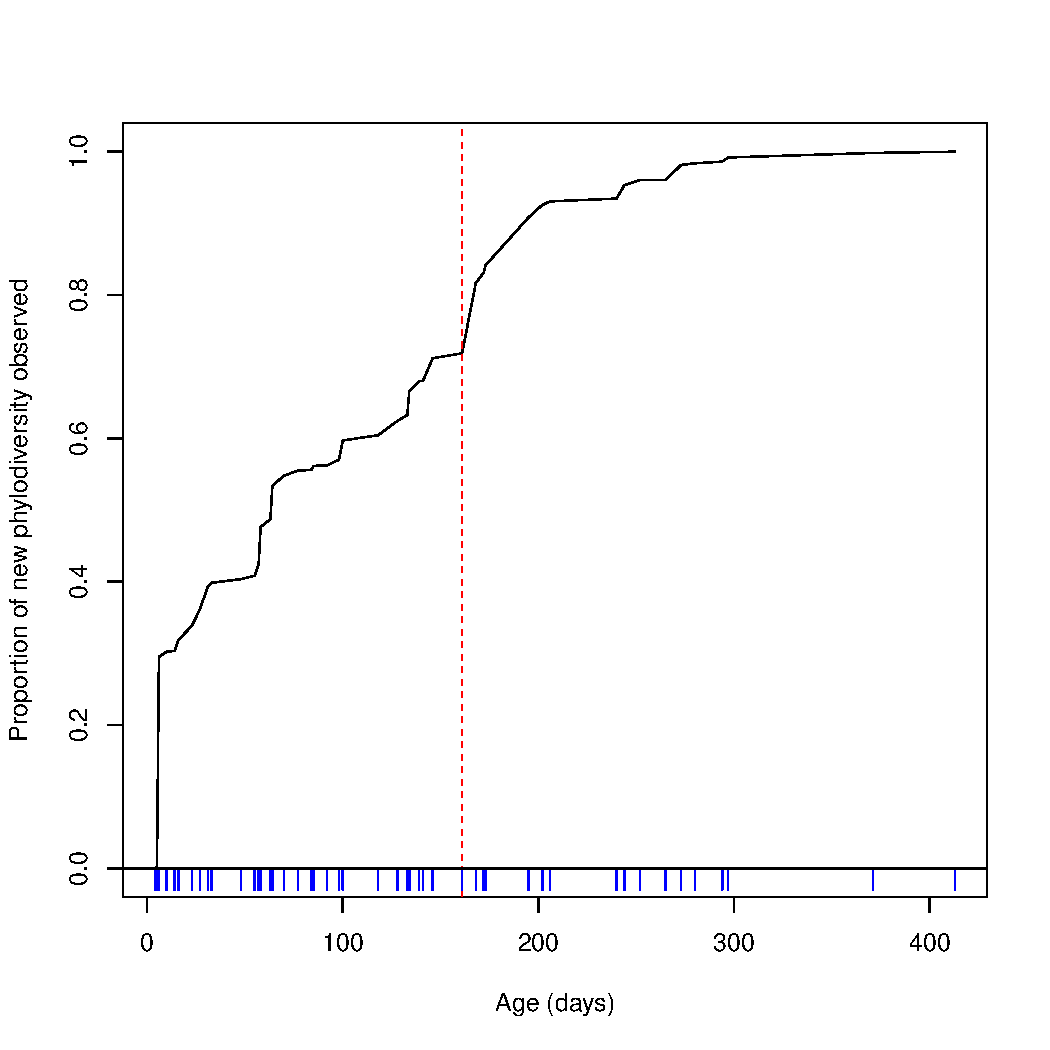
\includegraphics[scale=0.80]{figs/Fig_3.pdf}
\end{figure}
\textbf{Figure 3:}\label{sec:figure3} Empirical phylodiversity accumulation in the infant gut microbiome \cite{Koenig2011}. Phylodiversity increases sharply after day 161 of the infant’s life, then plateaus. This timing coincides with the day the subject began consuming baby formula. The times of sampling points are shown as vertical blue lines below the X-axis.
\newpage

\begin{figure}[t]
	\centering
	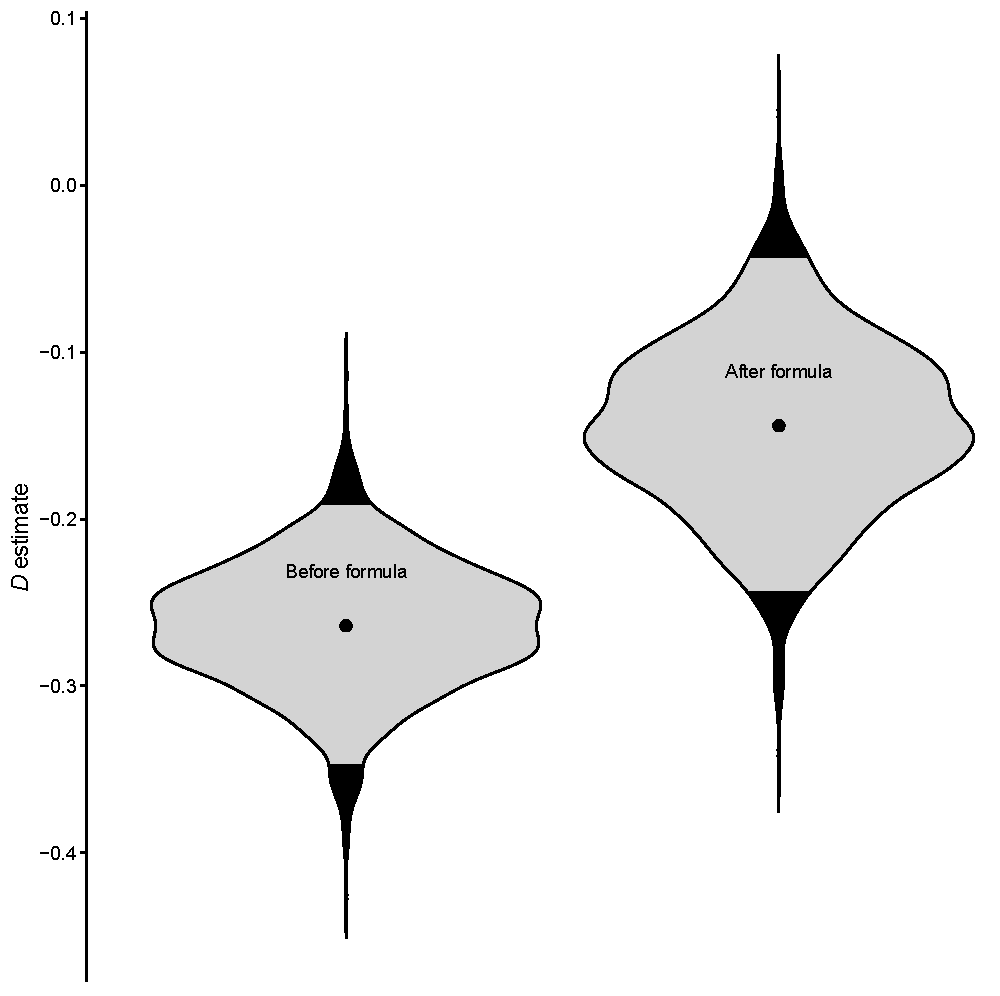
\includegraphics[scale=0.80]{figs/Fig_4.pdf}
\end{figure}
\textbf{Figure 4:}\label{sec:figure4} Dispersion parameter (\(D\)) estimates in the infant gut, pre-formula and during formula use. Formula use began on day 161, thus the first 160 days of the subject's life were analyzed separately. Community assembly was significantly underdispersed in the pre-formula data set, but was not significantly different from the neutral model during formula use (\(P = 0.107\)).
\newpage

}%close indentation stopper

% REFERENCES
\bibliography{refs}


% SUPPLEMENTAL MATERIAL
\newpage
\section{Supplemental Material}
{\parindent0pt % no indentation until closed
\begin{figure}[ht]
	\centering
	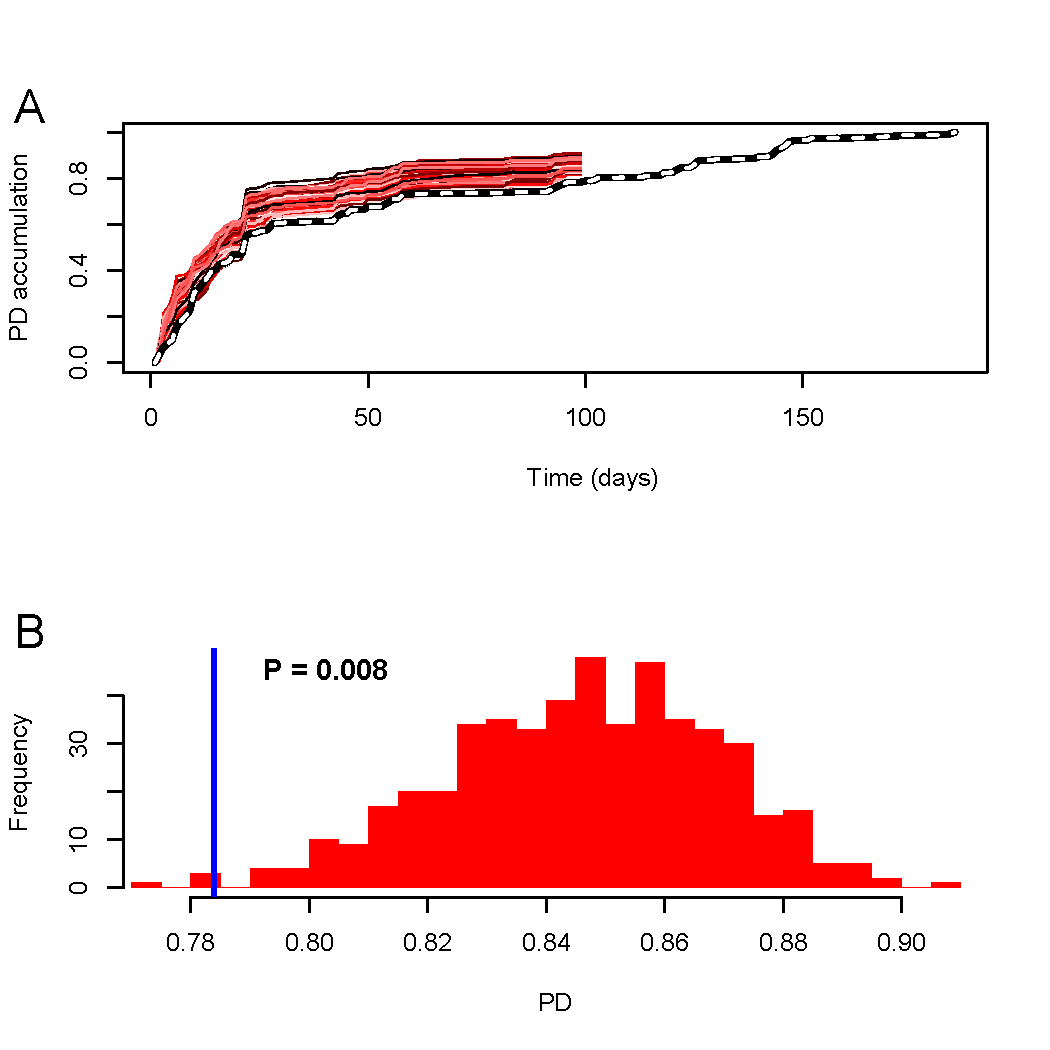
\includegraphics[scale=0.80]{figs/Fig_S1.pdf}
\end{figure}
\textbf{Supplemental Figure 1:}\label{sec:figureS1} Significance testing for the female feces data set. Plot A shows the empirical phylodiversity accumulation (dashed; same as \hyperref[sec:figure1]{Figure 1A}) but with neutral model surrogate data sets shown in different shades of red. These are produced by running the neutral model 500 times, to generate a distribution of phylodiversity values under \(D = 0\) (Plot B). As with all surrogate data sets, these are run until time \(m\) (see \hyperref[sec:parameterEstimation]{Parameter Estimation} section of Materials and Methods). Empirical phylodiversity at time \(m\) (blue line) is compared to the distribution of neutral model phylodiversities at time \(m\) (red histogram), and a \(P\)-value is calculated as the proportion of neutral phylodiversities more extreme than the empirical value. 
\newpage

\begin{figure}[t]
	\centering
	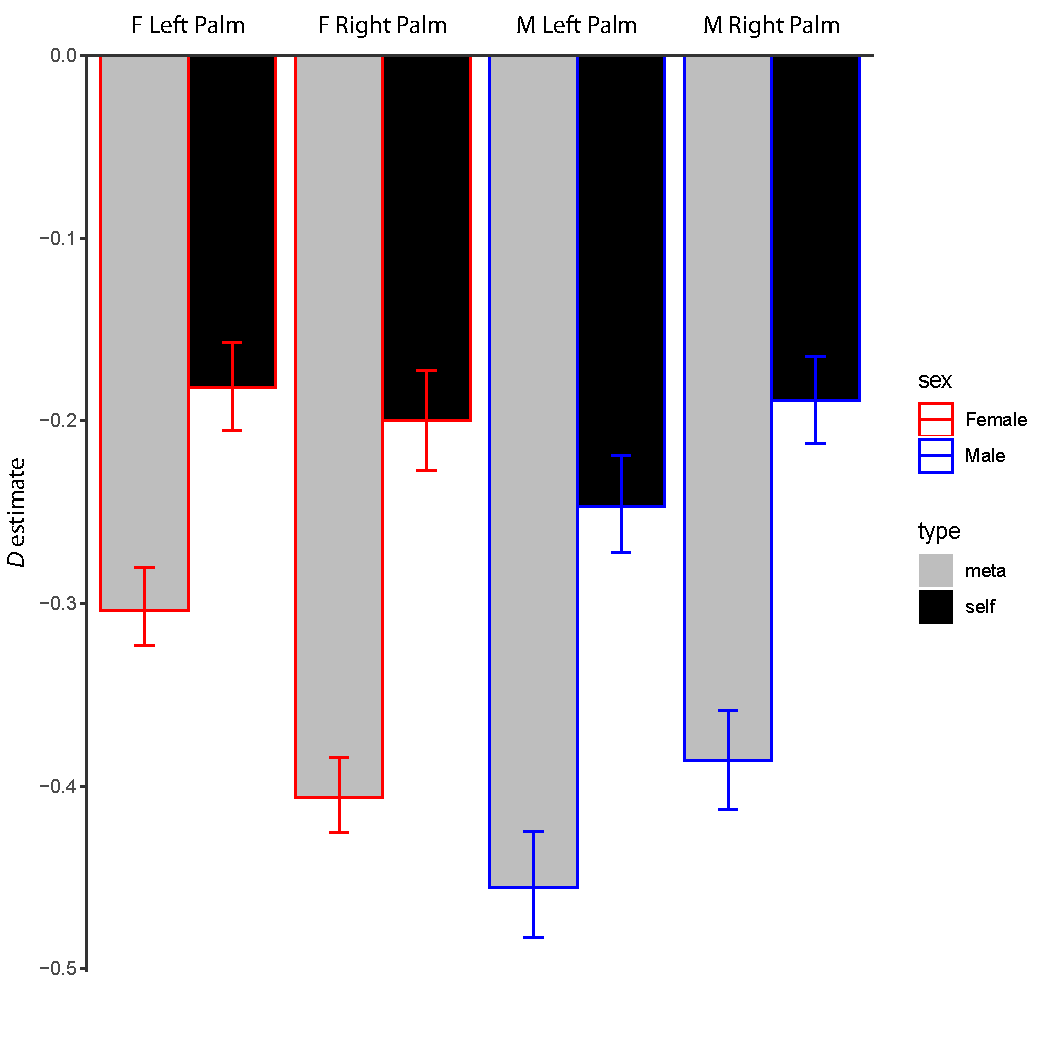
\includegraphics[scale=0.80]{figs/Fig_S2.pdf}
\end{figure}
\textbf{Supplemental Figure 2:}\label{sec:figureS2} Comparison of “self” vs “meta” model results from palm communities. “Self” (black) models were run identically to \hyperref[sec:figure2]{Figure 2}), but “meta” (gray) models were run where the species pool for each palm community surrogate data set was composed of all zOTUs observed across all four palm data sets. The difference between the “self” \(D\) estimate (generated above) and the “meta” \(D\) estimate (estimated with a metapopulation of zOTUs) is related to the exclusivity of arrivals into the community. In other words, if we were to estimate similar \(D\) values for both the “meta” and “self” analyses, the inclusion of extra species in the species pool would be of little importance to the model, and we would learn that it would make little difference to community assembly patterns if the species pool really was composed of the “meta” set.
\newpage

\begin{figure}[t]
	\centering
	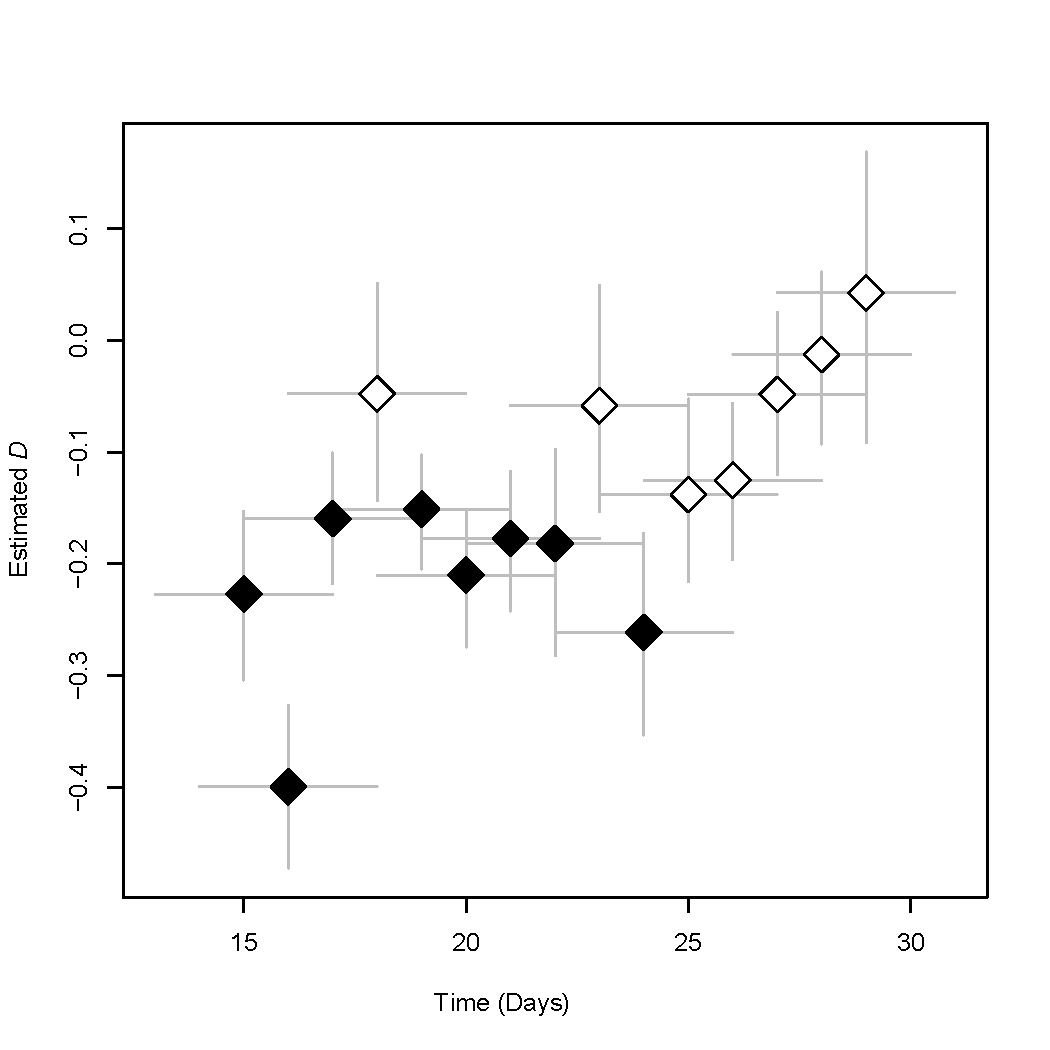
\includegraphics[scale=0.80]{figs/Fig_S3.pdf}
\end{figure}
\textbf{Supplemental Figure 3:}\label{sec:figureS3} Sliding window analysis of male right palm data over 19 consecutive samples. We ran our model on each window of 5 continuous days (15 windows), in order to see how \(D\) varied over time. We only conducted this analysis for the section of samples that were sampled every day, so that comparisons between windows would not be confounded by window size. This analysis was done to demonstrate a potential use case for our model, and not to test any specific hypothesis. Filled shapes represent windows that were significantly different than the neutral model. Vertical bars represent 95\% confidence intervals for \(D\) estimate, and horizontal bars represent window size.
\newpage

\begin{figure}[t]
	\centering
	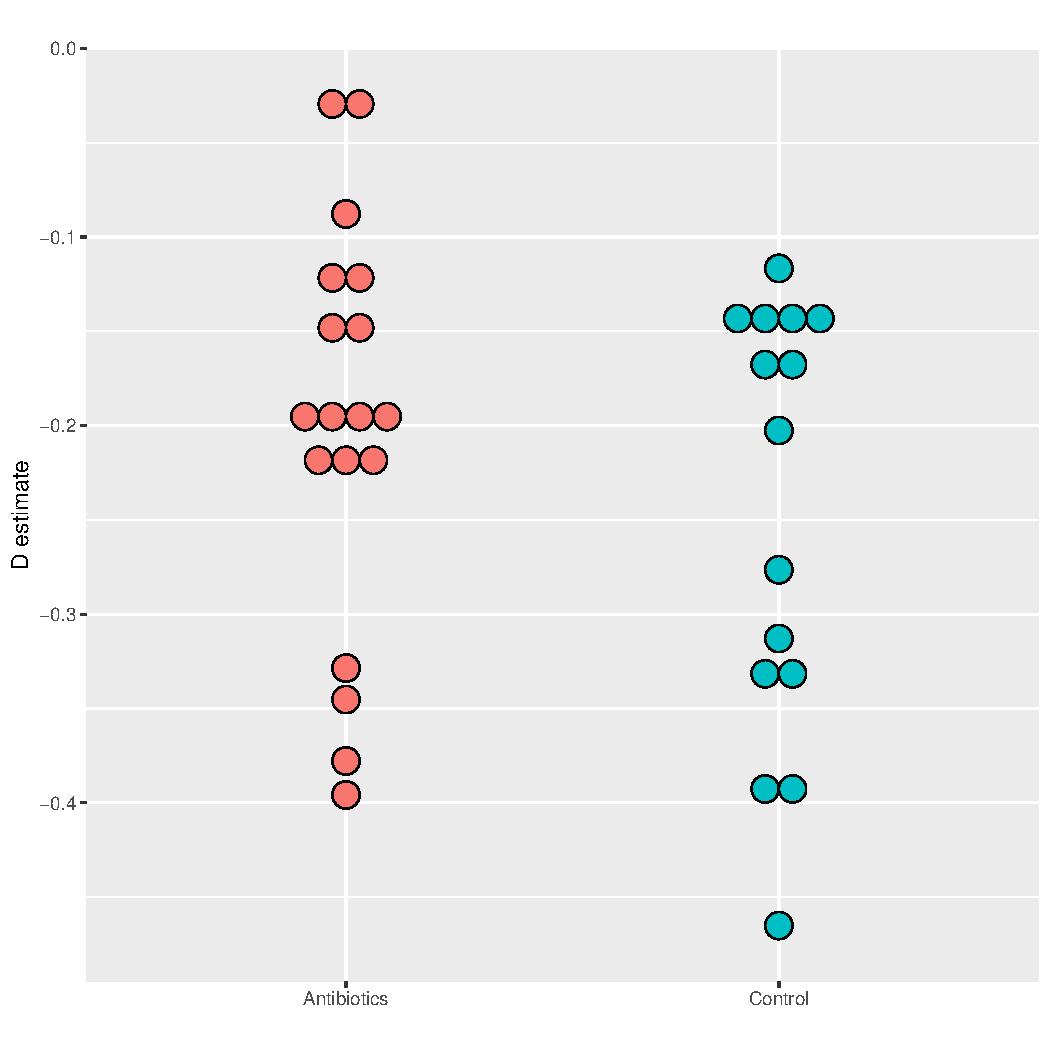
\includegraphics[scale=0.80]{figs/Fig_S4.pdf}
\end{figure}
\textbf{Supplemental Figure 4:}\label{sec:figureS4} \(D\) estimates of Finnish infant data sets. All but two subjects exhibited significant phylogenetic underdispersion. The two subjects that were not significantly different from the neutral model were both in the antibiotics cohort, which is comprised of infants that were treated with frequent antibiotics, almost all for ear infections. There was no significant difference between \(D\) values for the two groups. 
\newpage

\begin{figure}[t]
	\centering
	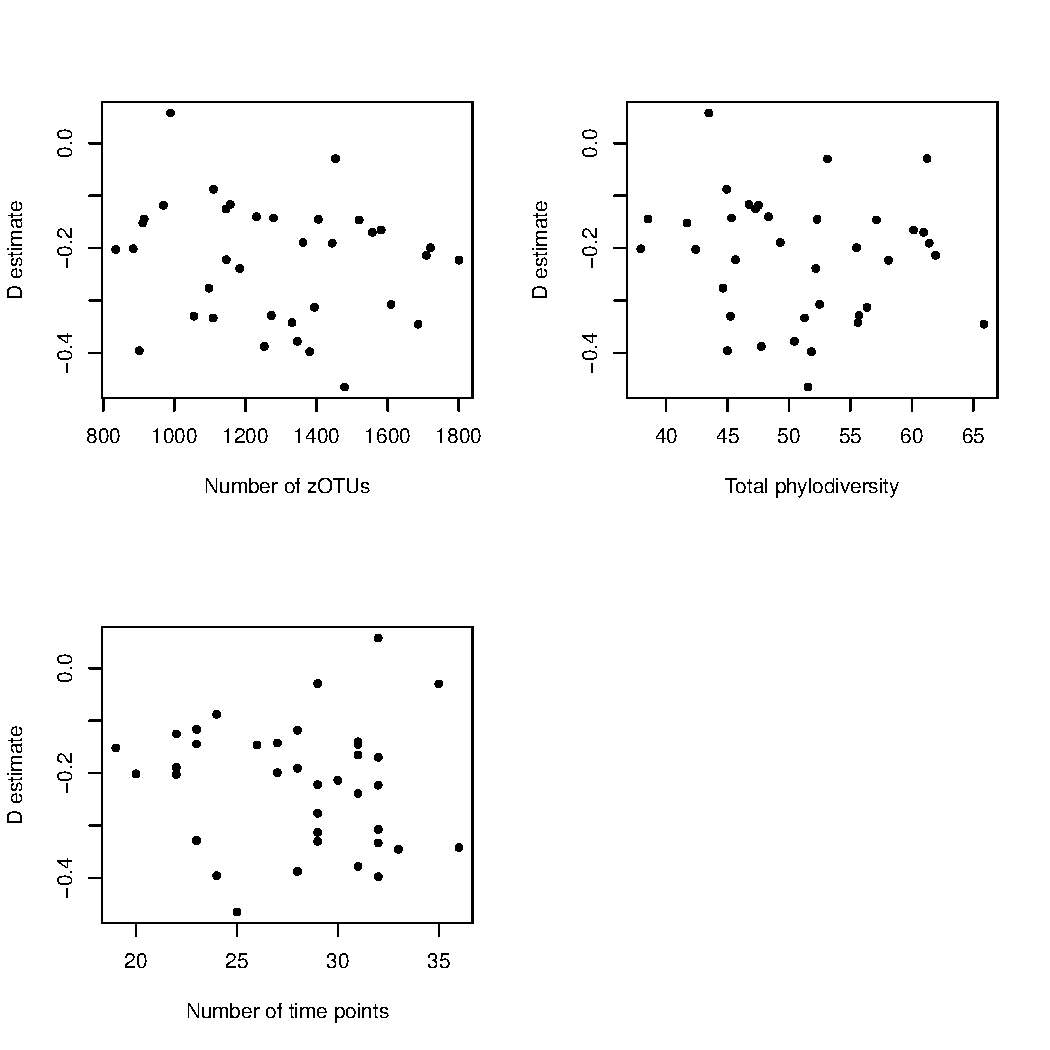
\includegraphics[scale=0.80]{figs/Fig_S5.pdf}
\end{figure}
\textbf{Supplemental Figure 5:}\label{sec:figureS5} Relationship of \(D\) estimate to total phylodiversity, zOTU richness, and number of time-points sampled for Finnish infant data. No statistically significant correlation was detected in any of these three analyses. 

}%close indentation stopper







\end{document}

